\documentclass{../source/zjureport}

\major{信息工程}
 \name{箫宇 }
\title{基于RV32I指令集的RISC-V微处理器设计}
\stuid{ }
\college{信息与电子工程学院}
\date{\today}
\lab{教11-400}
\course{计算机组成与设计}
\instructor{屈民军、唐奕}
\grades{}
\expname{基于RV32I指令集的微处理器设计}
\exptype{设计实验}
\partner{}

\begin{document}
    \makecover
    \makeheader

    \section{实验目的}
        \begin{enumerate}
            \item 熟悉RISC-V 指令系统。
            \item 了解提高CPU 性能的方法。
            \item 掌握流水线RISC-V 微处理器的工作原理。
            \item 理解数据冒险、控制冒险的概念以及流水线冲突的解决方法。
        \end{enumerate}
    
    \section{实验任务}
        \subsection{基本要求}
        设计一个流水线RISC-V 微处理器,具体要求如下所述。
            \subsubsection{至少运行下列RV32I 核心指令。}
                \begin{enumerate}
                    \item 算术运算指令:add、sub、addi
                    \item 逻辑运算指令:and、or、xor、slt、sltu、andi、ori、xori、slti、sltiu
                    \item 移位指令:sll、srl、sra、slli、srli、srai
                    \item 条件分支指令:beq、bne、blt、bge、bltu、bgeu
                    \item 无条件跳转指令:jal、jalr
                    \item 数据传送指令:lw、sw、lui、auipc
                    \item 空指令:nop
                \end{enumerate}
            \subsubsection{采用5 级流水线技术,对数据冒险实现转发或阻塞功能。}
            \subsubsection{在Nexys Video 开发系统中实现RISC-V 微处理器,要求CPU 的运行速度大于25MHz。}
        \subsection{扩展要求}
            \subsubsection{要求设计的微处理器还能运行lb、lh、ld、lbu、lhu、lwu、sb、sh 或sd 等字节、半字和双字数据传送指令。}
            \subsubsection{要求设计的CPU 增加异常(exception)、自陷(trap)、中断(interrupt)等处理方案。}
        
    \section{实验原理与各模块设计}
        \subsection{总体设计}
        流水线是数字系统中一种提高系统稳定性和工作速度的方法,广泛应用于高档CPU的架构中。根据RISC-V处理器指令的特点,将指令整体的处理过程分为取指令(IF)、指令译码(D)、执行〈EX)、存储器访问(MEM)和寄存器回写(WB)五级。如图\ref{流水线流水作业示意图}示,一个指令的执行需要5个时钟周期,每个时钟周期的上升沿来临时,此指令所代表的一系列数据和控制信息将转移到下一级处理。
        \begin{figure}[H]
            \centering
            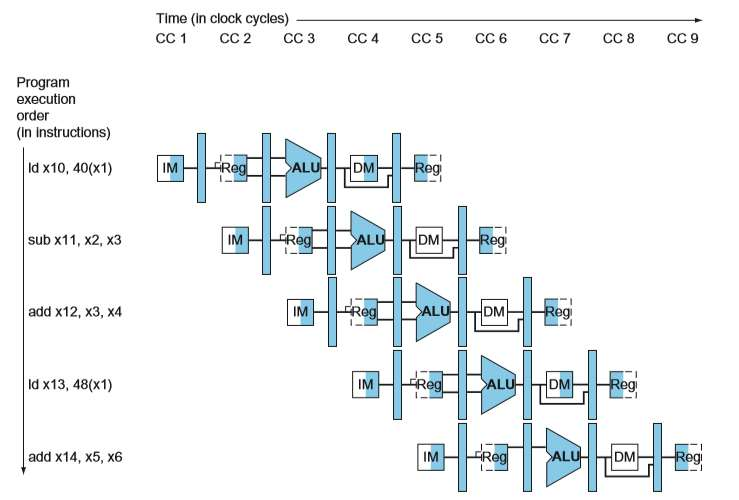
\includegraphics[]{figure/流水线流水作业示意图.jpg}
            \caption{流水线流水作业示意图}
            \label{流水线流水作业示意图}
        \end{figure}
        图\ref{流水线原理框图}所示为符合设计要求的流水线RISC-V微处理器的原理框图,采用五级流水线。由于在流水线中,数据和控制信息将在时钟周期的上升沿转移到下一级,所以规定流水线转移的变量命名遵守如下格式:名称_流水线级名称。如,在ID级指令译码电路〈decode)产生的寄存器写允许信号RegWrite在ID级、EX级、MEM级和WB级上的命名分别为RegWrite_id.RegWrite_ex .RegWrite_mem和RegWrite_wb。在顶层文件中,类似的变量名称有近百个,这样的命名方式起到了很好的识别作用。
        \begin{figure}[H]
            \centering
            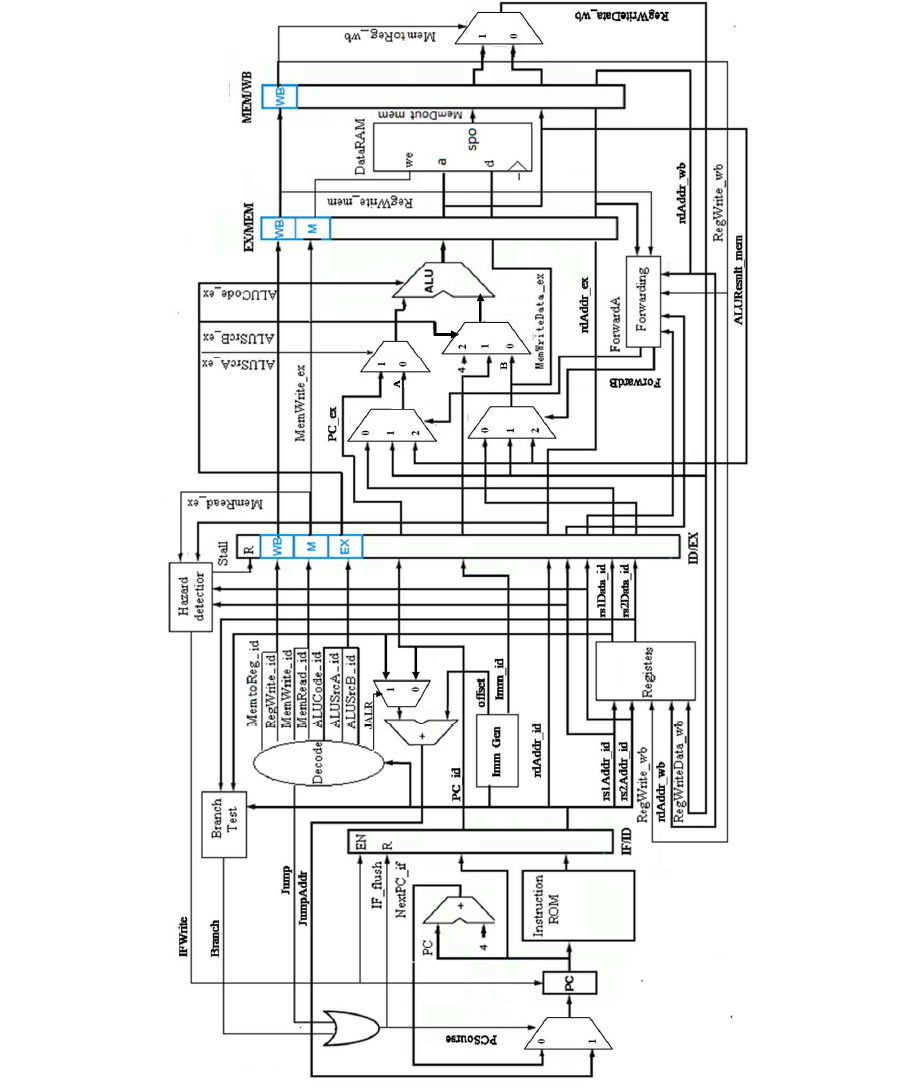
\includegraphics[width = \textwidth]{figure/流水线原理框图.png}
            \caption{流水线原理框图}
            \label{流水线原理框图}
        \end{figure}

        根据流水线不同阶段,将系统划分为IF、ID、EX 和MEM 四大模块,WB 部分功能电路非常简单,可直接在顶层文件中设计。另外,系统还包含IF/ID、ID/EX、EX/MEM、MEM/WB 四个流水线寄存器。

        \subsection{指令译码ID模块的设计}
        指令译码模块的主要作用是从机器码中解析出指令,并根据解析结果输出各种控制信号。ID 模块主要由指令译码(Decode)、寄存器堆(Registers)、冒险检测、分支检测和加法器等组成。ID 模块的接口信息如图\ref{ID模块的输入输出引脚说明}所示。
        \begin{figure}[H]
            \centering
            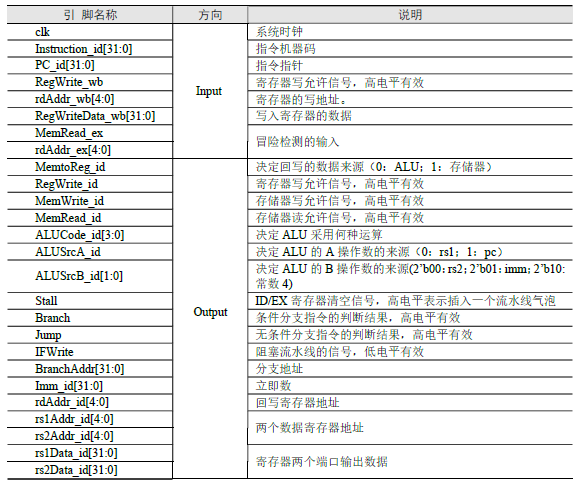
\includegraphics[]{figure/ID模块的输入输出引脚说明.png}
            \caption{ID模块的输入/输出引脚说明}
            \label{ID模块的输入输出引脚说明}
        \end{figure}

            \subsubsection{寄存器堆(Registers)子模块的设计}
            寄存器堆由32个32位宽的寄存器组成,并且寄存器x0的值始终为0值。同时因为需要解决三阶数据相关的数据转发问题,所以需要令其具有Read After Write特性。具体的实现电路如图\ref{寄存器堆}所示
            \begin{figure}[H]
                \centering
                \begin{minipage}[t]{0.48\textwidth}
                    \centering
                    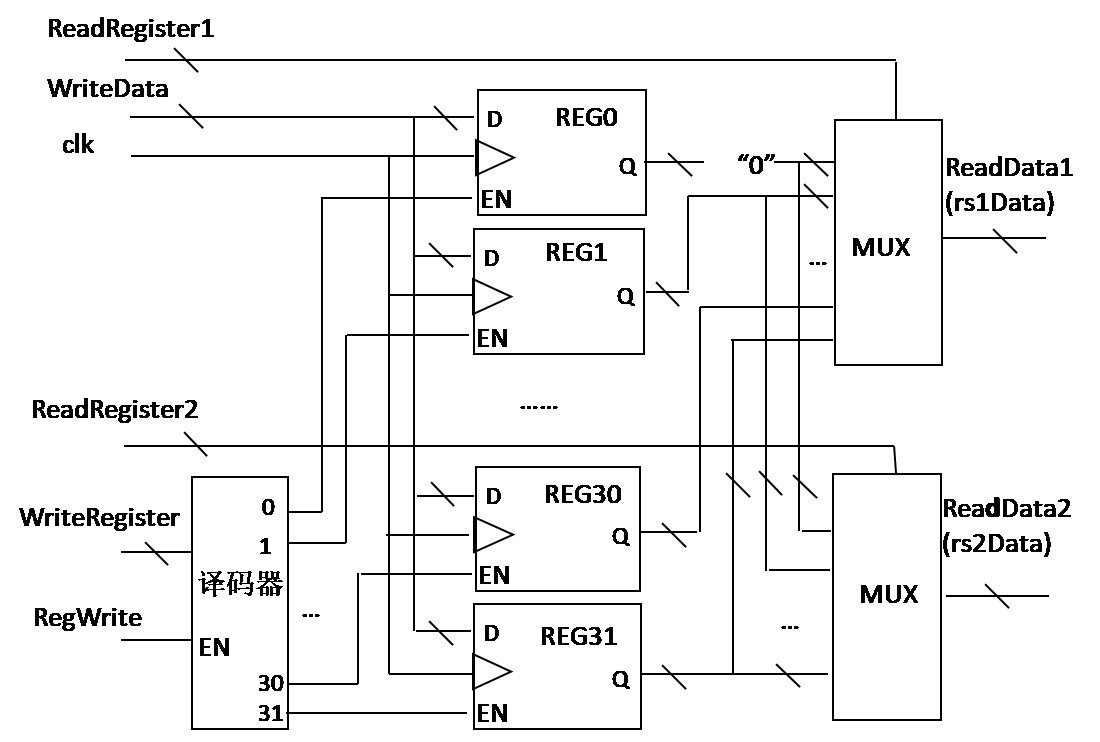
\includegraphics[width = \textwidth]{figure/寄存器堆的原理框图.jpg}
                    \caption*{寄存器堆的原理框图}
                \end{minipage}
                \begin{minipage}[t]{0.48\textwidth}
                    \centering
                    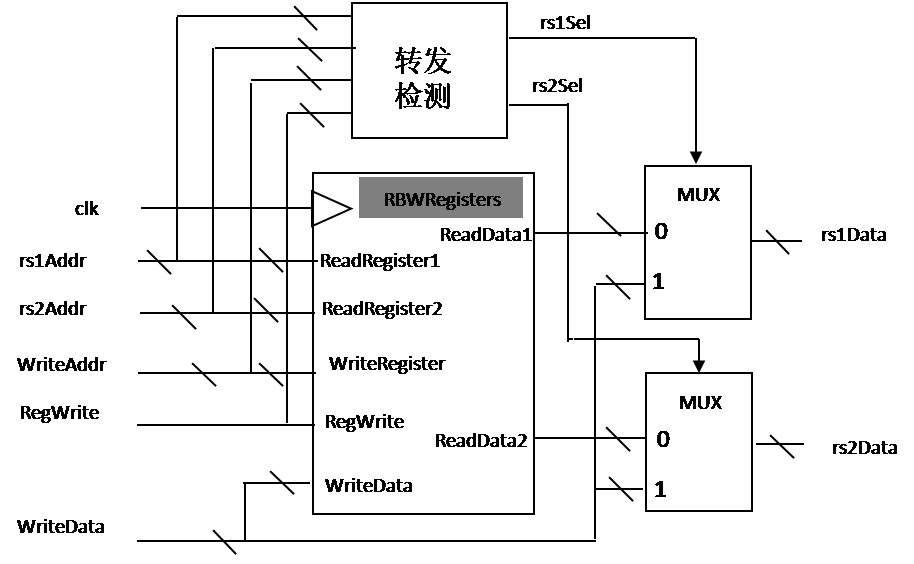
\includegraphics[width=\textwidth]{figure/具有RAW特性寄存器堆的原理框图}
                    \caption*{具有Read After Write特性寄存器堆的原理框图}
                \end{minipage}
                \caption{寄存器堆}
                \label{寄存器堆}
            \end{figure}
            如图\ref{寄存器堆}书写寄存器堆模块的Verilog代码,具体实现请参见Solution中RAWRegisters.v文件,核心语句如代码\ref{寄存器堆}所示:
            \begin{lstlisting}[
                caption = 寄存器堆,
                language = Verilog,
                label = 寄存器堆
            ]
            //assign the value of temprary readData
            assign ReadData1 = (rs1Addr == 5'b0)?31'b0:regs[rs1Addr];
            assign ReadData2 = (rs2Addr == 5'b0)?31'b0:regs[rs2Addr];
        
            //assign the values of select signal
            assign rs1Sel = RegWrite & (WriteAddr != 0) & (WriteAddr == rs1Addr);
            assign rs2Sel = RegWrite & (WriteAddr != 0) & (WriteAddr == rs2Addr);
        
            //write data into regs
            always @(posedge clk) begin
                if(RegWrite) regs[WriteAddr] <= WriteData;
            end
        
            //if need forward , choose WriteData as output,else choose the data from regs
            assign rs1Data = (rs1Sel == 1)?WriteData:ReadData1;
            assign rs2Data = (rs2Sel == 1)?WriteData:ReadData2;
            \end{lstlisting} 
            
            \subsubsection{指令译码(包括立即数产生电路)子模块的设计}
            这一模块主要是依据输入的指令产生对应的控制信号,同时产生应有的立即数Imm以及偏移量offset供流水线的控制使用。这一模块采用组合电路进行设计。

            实现思路主要为先将指令按域进行划分,然后依据op的值判断出输入指令的类型,随后按照不同指令类型的定义产生应有的控制信号以及立即数(偏移量)。

            代码主要见Solution中Decode.v文件。

            \subsubsection{分支检测电路的设计}
            此模块主要是为了判断出分支条件是否成立,虽然在Verilog中可以采用运算符号进行描述,但是需要注意有符号数和无符号数的处理是有着不同的,此次实验中我们采用32位快速加法器进行实现。实现步骤如下:

            首先利用加法器实现rs1Data+(~rs2Data)+1(即rs1Data-rs2Data),设结构为sum[31:0],列出真值表我们可以得出代码\ref{分支判断核心语句}中的表达式,分支判断模块的其余代码请参见Solution中的testBranch.v文件。
            \begin{lstlisting}[
                language = Verilog,
                caption = 分支判断核心语句,
                label = 分支判断核心语句
            ]
    isLT = rs1Data[31] && (~rs2Data[31]) || (rs1Data[31]~^rs2Data[31]) && sum[31];//有符号数
    isLTU = (~rs1Data[31]) && rs2Data[31] || (rs1Data[31]~^rs2Data[31]) && sum[31];//无符号数
            \end{lstlisting}

            \subsubsection{冒险检测功能电路的设计}
            分析可得,冒险成立的条件有以下两条:
            \begin{enumerate}
                \item 前一条指令为lw指令
                \item 两条指令读写同一个寄存器
            \end{enumerate}
            满足以上两个条件是应当清空ID/EX寄存器并且阻塞流水线ID级、IF级流水线,所以会产生如下两个控制信号。
            \begin{lstlisting}[
                language = Verilog
            ]
    assign Stall = ((rdAddr_ex == rs1Addr_id)||(rdAddr_ex == rs2Addr_id)) && MemRead_ex;
    assign IFWrite = ~Stall;
            \end{lstlisting}

        \subsection{执行模块设计}
        执行模块主要由ALU子模块,数据前推电路以及数据选择器构成,具体数据流向可以参考图\ref{流水线原理框图}中的EX模块。执行模块的输入输出信息如图\ref{EX模块输入输出引脚说明}所示。
        \begin{figure}[H]
            \centering
            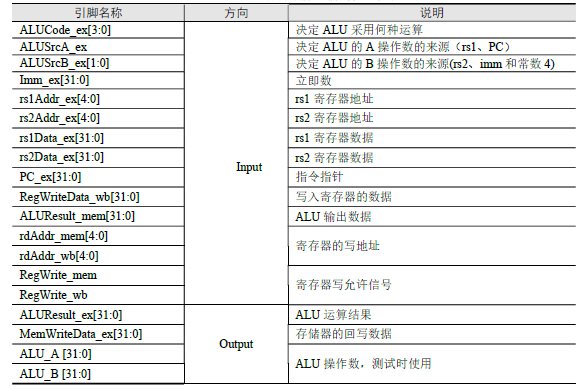
\includegraphics[width = 0.85\textwidth]{figure/执行模块输入输出引脚说明.png}
            \caption{EX模块的输入输出引脚说明}
            \label{EX模块输入输出引脚说明}
        \end{figure}

            \subsubsection{ALU子模块的设计}
            ALU模块提供CPU的基础运算能力,比如加、减、移位、与或、比较等。

            此模块接收两个操作数以及一个控制信号ALUCode,控制信号用于控制ALU执行什么操作。输出为一个32位的ALUResult。

            为了提高运算速度,一方面首先我们让ALU并行执行所有的运算类型,然后根据ALUCode的不同选择不同的运算结果。另一方面我们提高32位加法器的运算速度,此次实验中我选择了进位选择加法器。

            此模块中尤其需要注意的为进行算术右移操作时,Verilog中的算术右移操作符'>>>'被移位的对象只能够是reg类型,所以需要声明一个中间变量对其进行算术右移,代码如下:
            \begin{lstlisting}
                reg signed[31:0] A_reg;
                always@(*) begin A_reg = A; end
            \end{lstlisting}

            此子模块的代码详情可见Solution中的ALU.v文件。

            \subsubsection{数据前推电路}
            此部分电路主要由数据选择器以及产生数据选择器控制地址信号的ForwardA与ForwardB确定。首先按照实验手册中的要求产生正确的ForwardA与ForwardB信号,然后按照图\ref{流水线原理框图}中EX模块中的数据前推部分连接信号。

            \subsection{数据存储模块(DataRAM)的设计}
            此模块采用Xilinx的IP内核实现,此处我们生成了一个空间为$64\times32$bit的单端口RAM,输出为组合输出。因为容量为$64\times32$bit,所以存储器地址共6位,所以将地址位与ALUResult_mem[7:2]连接。

        \subsection{取指令模块(IF)的设计}
        IF模块主要由指令指针寄存器(PC),指令存储器子模块(Instruction ROM),指令指针选择器(MUX)和一个32位加法器组成,IF模块的接口信息如图\ref{IF模块接口信息}所示。
        \begin{figure}[H]
            \centering
            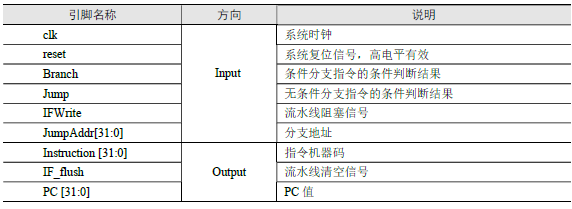
\includegraphics[]{figure/IF接口信息.png}
            \caption{IF模块的输入/输出引脚说明}
            \label{IF模块接口信息}
        \end{figure}
        其中指令指针寄存器用于存储当前PC值,由一个D触发器构成,以控制信号IFWrite作为触发器的使能信号确认是否需要更新PC值。
        
        指令存储器模块用于存储代码的所有指令。

        指令指针选择器根据Decode模块解码出来的控制信号确认选择原PC值加4或是选择跳转之后的PC值,以此方式实现指令的跳转。

        32位加法器用于实现PC值的自增。

        此模块的具体实现请参加Solution中的IF.v文件,此处不再赘述。

        \subsection{流水线寄存器的设计}
        流水线寄存器的作用为将流水线的各个部分却分开来,一共有IF/ID,ID/EX,EX/MEM,MEM/WB四组。
        
        其中IF/ID这一组寄存器要求带有同步清零功能,并且因为在发生数据冒险时需要阻塞IF/ID寄存器,所以其还需要带有保持功能(具有使能EN信号输入)

        ID/EX流水线寄存器需要带有同步清理功能,因为在发生数据冒险时需要将其清空。

        而EX/MEM,MEM/WB两个流水线寄存器则只是普通的D型触发器。

        因为每一组寄存器都有许多变量,所以如果采用单输入的D触发器会使编程工作变得繁琐起来,所以我在书写这一部分时选择了每一组寄存器都实例化一个多输入的D触发器。

        \subsection{顶层设计}
        顶层设计只需要将前面各个模块按照图\ref{流水线原理框图}进行连接即可。连接的过程中注意按照信号所属层级进行命名,以此方便区分不同阶段的信号。

    \section{主要仪器设备}
    \begin{enumerate}
        \item 装有 Vivado和 ModelSim SE软件的计算机。
        \item Nexys Video开发板一套。
        \item 带有HDMI接口的显示器一台。
    \end{enumerate}

    \section{实验结果}
        \subsection{Decode模块}
            \subsubsection{仿真图}
            \begin{figure}[H]
                \centering
                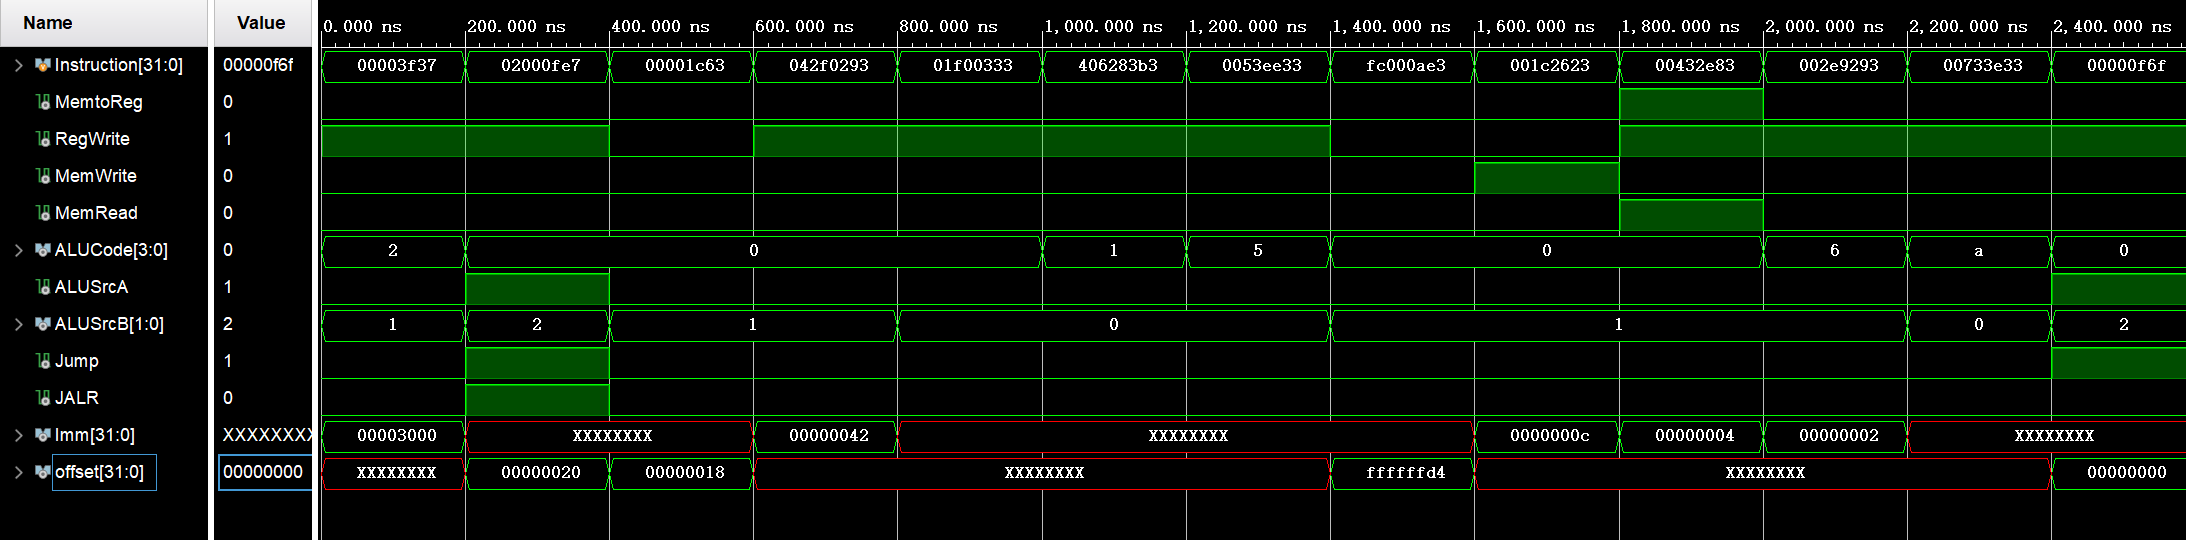
\includegraphics[width = 0.98\textwidth]{figure/decode.png}
                \caption{Decode模块仿真图}
            \end{figure}

            \subsubsection{仿真结果分析}
            从左到右依次手动译码每条指令得到以下结果:
            \begin{enumerate}
                \item lui x30, 0x3000, 为U型,输出应为Imm = 0x0000_3000,offset无意义, ALUCode=4'd2,ALUSrcA=0, ALUSrcB=2'b01, LUI指令需要回写,RegWrite=1,波形显示正确。
                \item ja1r X31,1ater(X0),为I型,输出应为Imm无意义,offset=0x0000_0020,ALUCode=4'd0,ALUSrcA=1,ALUSrcB=2'b10,JALR=1,Jump=1,JALR指令需要回写,RegWrite=1,波形显示正确。
                \item bne X0,X0,end , 为SB型 , 输出应为Imm无意义 , offset=0x0000_0018 , ALUCode=4'd0,  ALUSrcA=0 , ALUSrcB=2'b01 , BNE指令不需要回写 , RegWrite=0 , 波形显示正确。
                \item addi X5,X30,42,为I型,输出应为Imm =0x0000_0042,offset无意义,ALUCode=4'd0,ALUSrcA=0,ALUSrcB=2'b01,ADDI指令需要回写,RegWrite=1,波形显示正确。
                \item add X6,X0,X31,为R型,输出应为Imm无意义,offset无意义,ALUCode=4'd0,ALUSrcA=0,ALUSrcB=2'b00,ADD指令需要回写,RegWrite=1,波形显示正确。
                \item sub X7,X5,X6,为R型,输出应为Imm无意义,offset无意义,ALUCode=4'd1,ALUSrcA=0,ALUSrcB=2'b00,SUB指令需要回写,RegWrite=1,波形显示正确。
                \item or X28,X7,X5,为R型,输出应为Imm无意义,offset无意义,ALUCode=4'd5,ALUSrcA=0,ALUSrcB=2'b00,OR指令需要回写,RegWrite=1,波形显示正确。
                \item beq X0, X0, ear1ier,为SB型,输出应为Imm无意义,offset=0xffff_ffd4,ALUCode=4'd0,ALUSrcA=0,ALUSrcB=2'b01,BEQ指令不需要回写,RegWrite=0,波形显示正确。
                \item sw X28,0C(X0),为S型,输出应为Imm=0x0000_000c, offset无意义, ALUCode=4'd0 , ALUSrcA=0, ALUSrcB=2'b01,MemWrite=1,波形显示正确。
                \item lw X29,04(X6),为I型,输出应为Imm=0x0000_0004, offset无意义,ALUCode=4'd0, ALUSrcA=0, ALUSrcB=2'b01, MemRead=1,MemtoReg=1,RegWrite=1,波形显示正确。
                \item sll X5,X29,2,为I型,输出应为Imm=0x0000_0002,offset无意义 , ALUCode=4'd6 , ALUSrcA=0 , ALUSrcB=2'b01 , RegWrite=1,波形显示正确。
                \item sltu X28,X6,X7,为R型,输出应为Imm无意义,offset无意义,ALUCode=4'd10, ALUSrcA=0, ALUSrcB=2'b00 , RegWrite=1,波形显示正确。
                \item jal X31,done , 为UJ型 , 输出应为Imm无意义 , offset=0x0000_0000 , ALUCode=4'd1 ,  ALUSrcA=1 ,ALUSrcB=2'b10 ,SUB指令需要回写,RegWrite=1,波形显示正确。
            \end{enumerate}

            由上述分析可知,Decode模块仿真结果正常。


        \subsection{ALU模块}
            \subsubsection{完整仿真图}
            \begin{figure}[H]
                \centering
                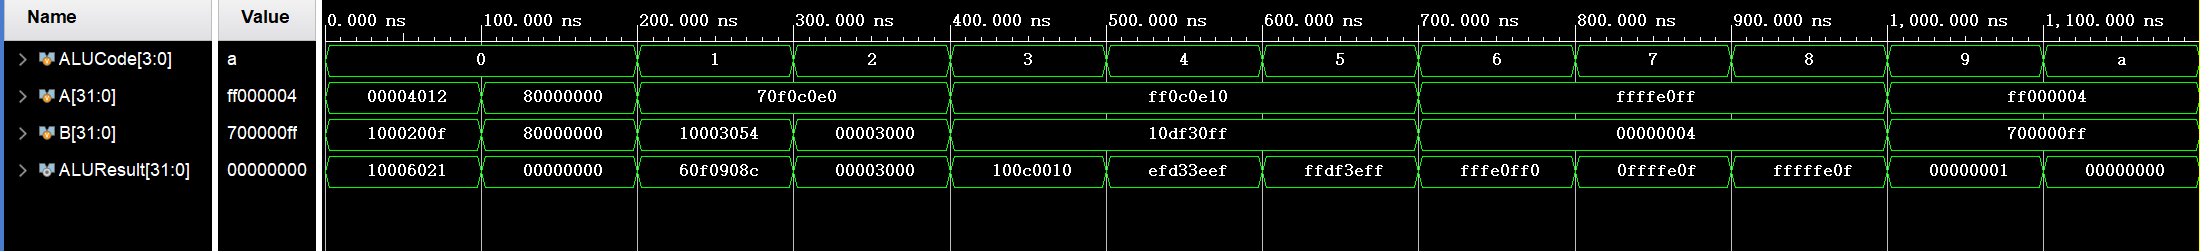
\includegraphics[width = 0.98\textwidth]{figure/ALU完整仿真图.png}
                \caption{ALU完整仿真图}
            \end{figure}

            \subsubsection{仿真图分析}
            \begin{figure}[H]
                \centering
                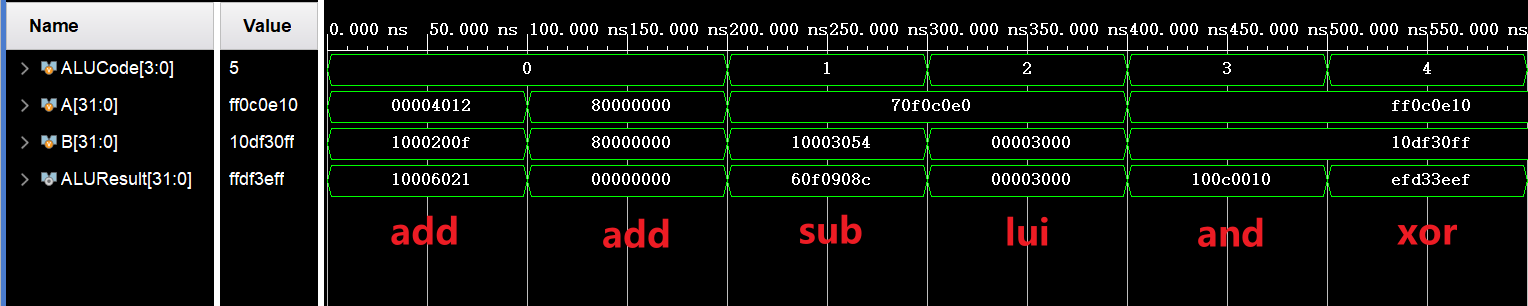
\includegraphics[width = 0.98\textwidth]{figure/ALU_1.png}
                \caption{ALU前半部分}
            \end{figure}
            \begin{figure}[H]
                \centering
                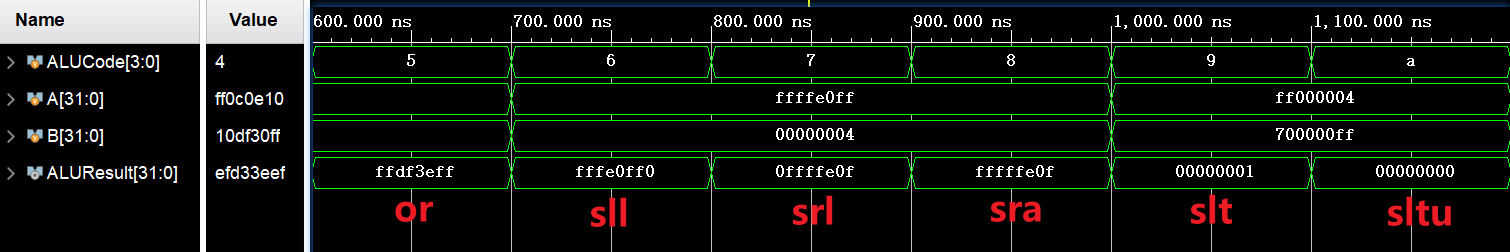
\includegraphics[width = 0.98\textwidth]{figure/ALU_2.png}
                \caption{ALU后半部分}
            \end{figure}
            在仿真图中已经标出了对应时间段的ALUCode对应操作,按照操作进行简单的计算即可证明ALU部分工作正常。
            
        \subsection{IF模块}
            \subsubsection{完整仿真结果}
            \begin{figure}[H]
                \centering
                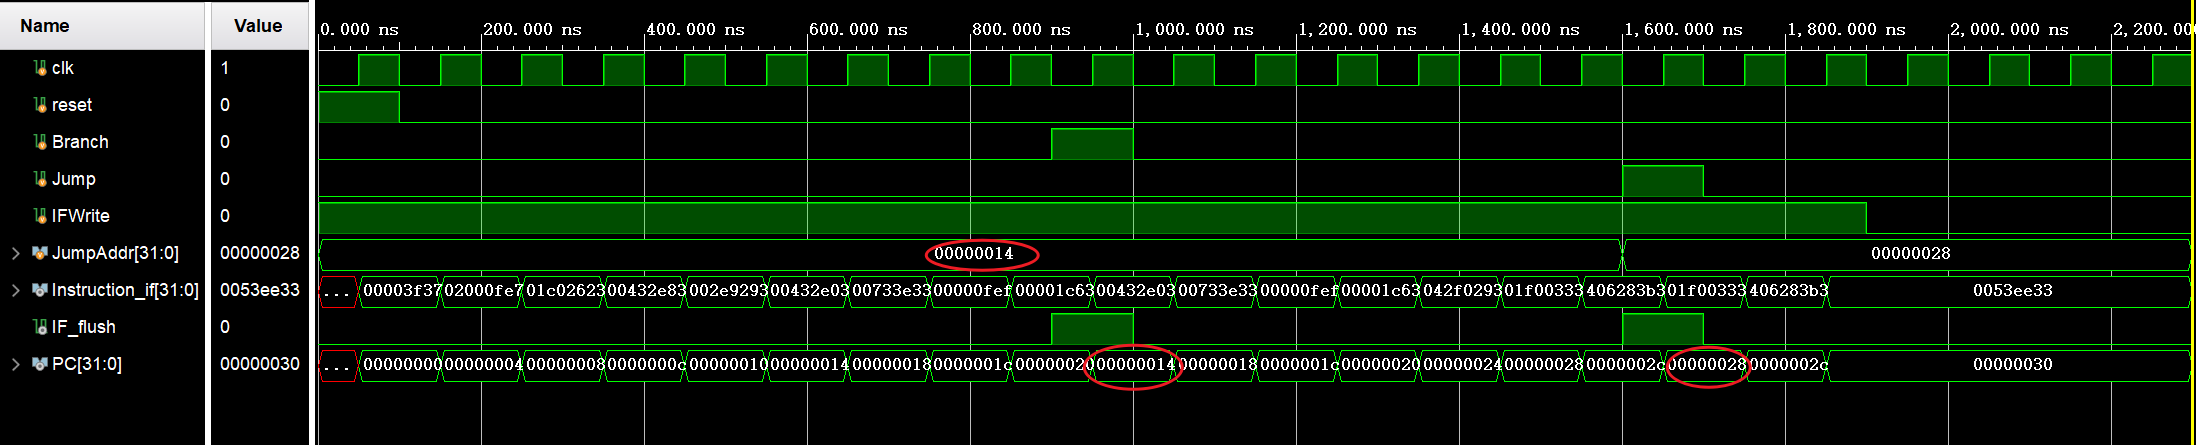
\includegraphics[width = 0.98\textwidth]{figure/IF.png}
                \caption{IF模块仿真结果}
            \end{figure}

            \subsubsection{结果分析}
            \begin{figure}[H]
                \centering
                \begin{minipage}[t]{0.48\textwidth}
                    \centering
                    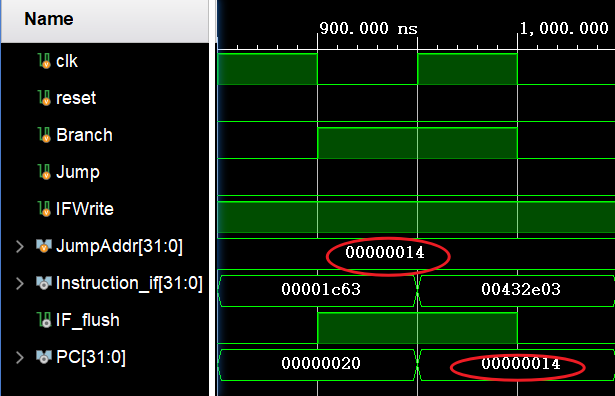
\includegraphics[width = \textwidth]{figure/IF局部1.png}
                    \caption*{IF局部图1}
                \end{minipage}
                \begin{minipage}[t]{0.48\textwidth}
                    \centering
                    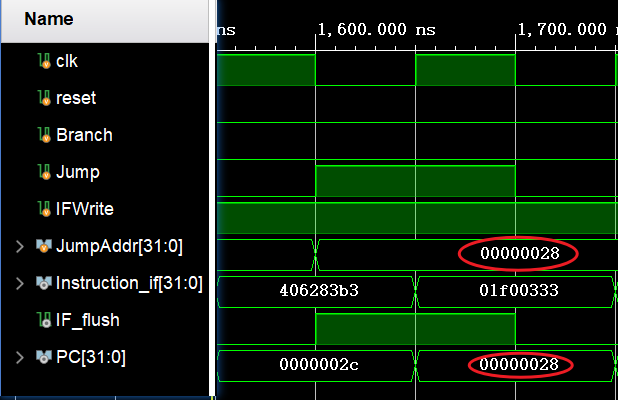
\includegraphics[width=\textwidth]{figure/IF局部2.png}
                    \caption*{IF局部图2}
                \end{minipage}
                \caption{IF局部分析}
                \label{IF局部图}
            \end{figure}

            通过分析上述图\ref{IF局部图}中两个两个局部图可以看出,当控制信号Branch或者Jump为1是,PC值能够实现正确跳转,而当两个控制信号均为0是,PC值则依次递增,说明IF模块运行正常。

        \subsection{CPU顶层}
            \subsubsection{仿真图像}
            \begin{figure}[H]
                \centering
                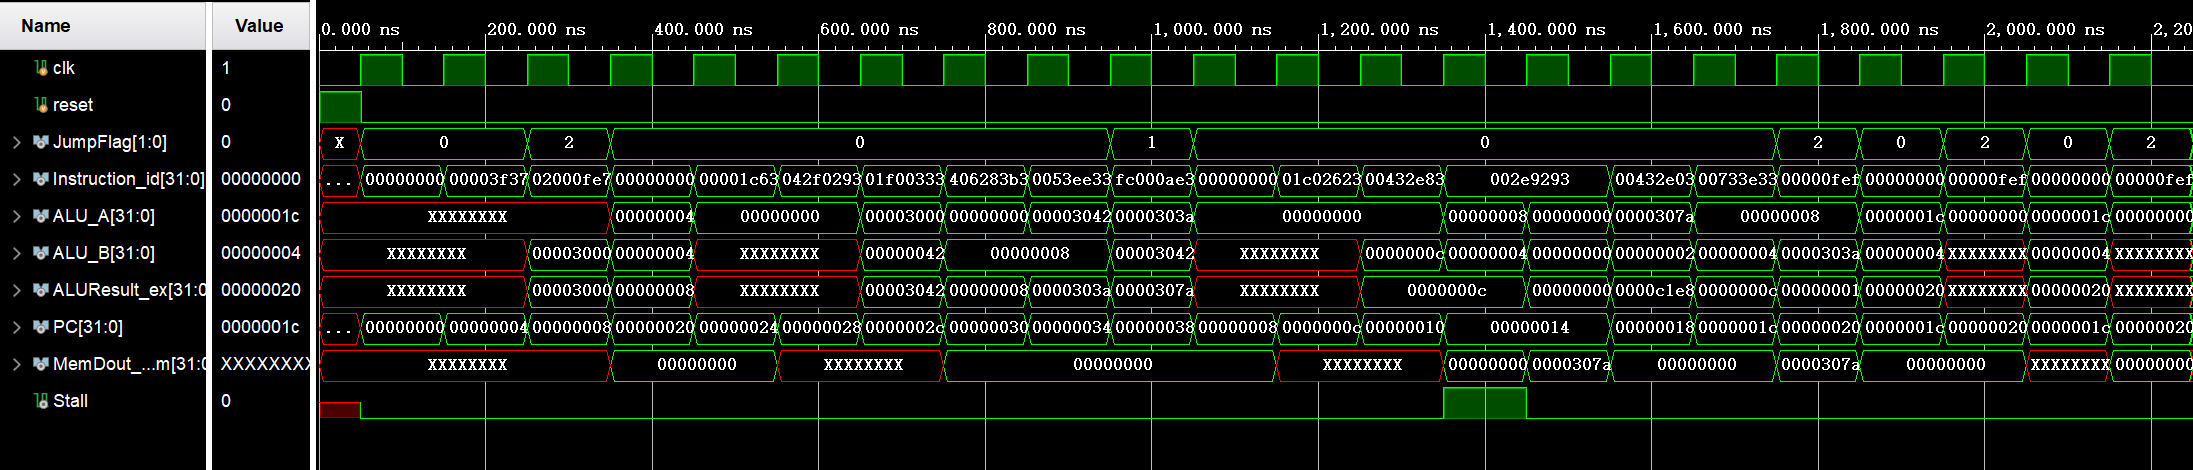
\includegraphics[width = 0.98\textwidth]{figure/顶层.png}
                \caption{CPU顶层仿真结果}
                \label{测试结果}
            \end{figure}

            \begin{figure}[H]
                \centering
                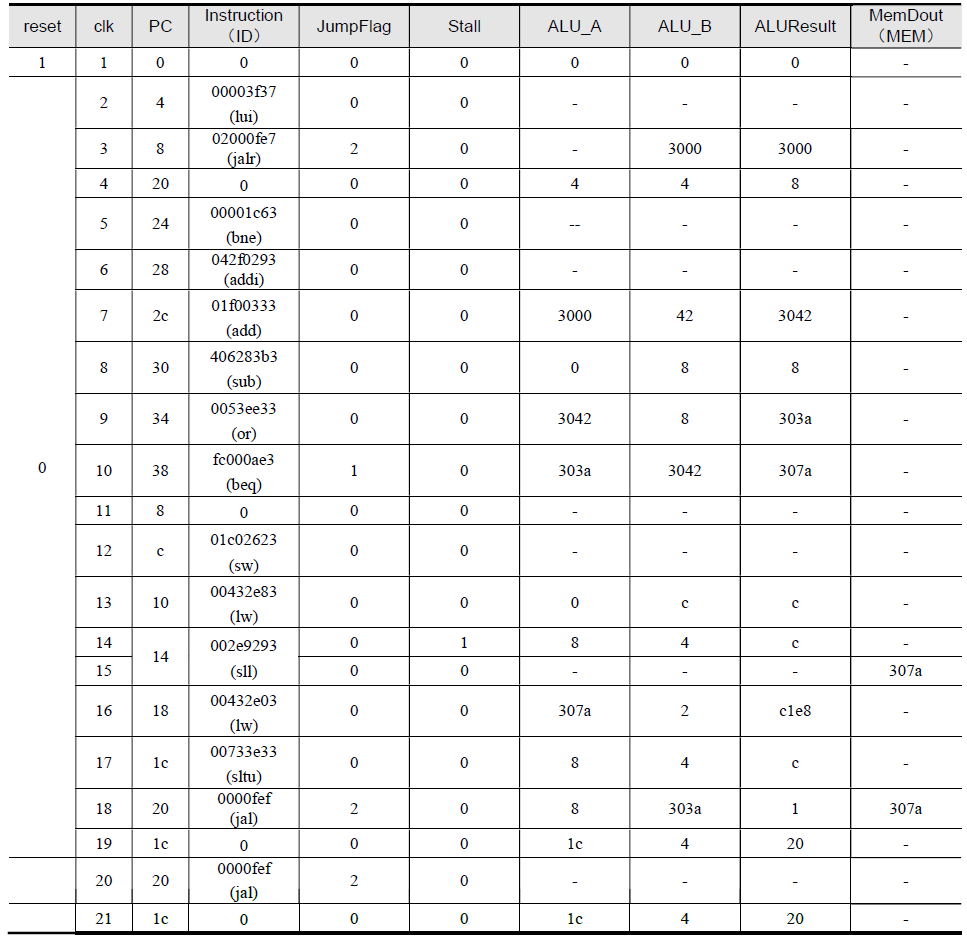
\includegraphics[width = 0.8\textwidth]{figure/测试结果.png}
                \caption{应有的测试结果}
                \label{应有结果}
            \end{figure}

            \subsubsection{结果分析}
            依次对比图\ref{测试结果}与图\ref{应有结果},可以发现仿真结果中每个周期内各个信号的取值与应有结果相同,由此可以说明仿真结果正确。

        \subsection{上板验证}
        \begin{figure}[H]
            \centering
            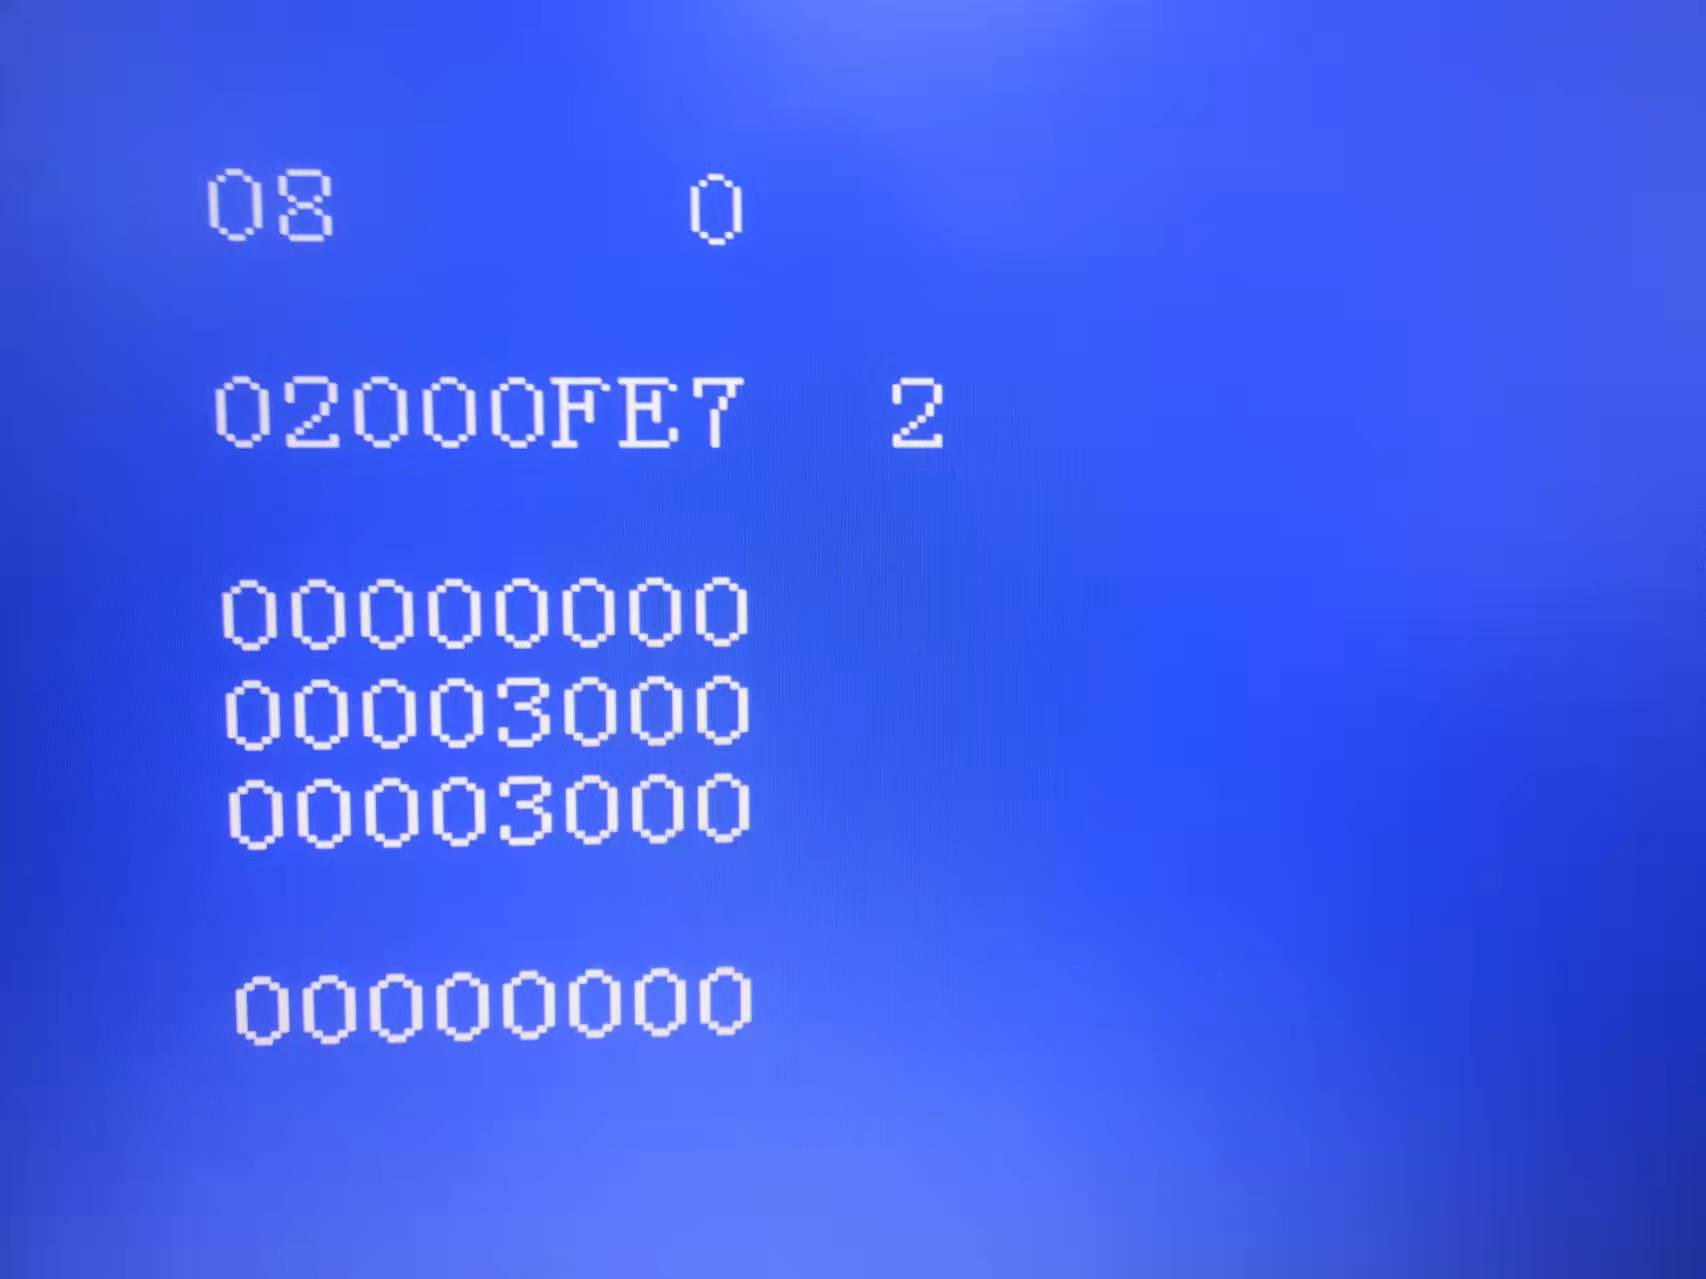
\includegraphics[width = 0.5\textwidth]{figure/上板结果.jpg}
            \caption{上板结果}
        \end{figure}

    
    \section{问题记录}
        \begin{enumerate}
            \item 文件没有做好备份,在实验做到一半的时候因为某些原因永久性删除了工程代码,导致最后耗费了比较多的时间重新写大作业。在第二次写的时候我吸取了上一次的教训,每写完一部分就将本地的代码与Github云端进行一次备份。
            \item 在设计 ALU的时候遇到 Binvert位扩展的问题,百度得到了结果,应该是{32{Binvert}}形式,最外面一定要有花括号。本次实验用到了很多数据位扩展的知识。
            \item IF/ID级寄存器的重置清零端传入的信号我最初单纯认为是reset,最后通过查看图\ref{流水线原理框图}后发现应该传入的值为IF_flush|reset。只有这样才能够达到在发生数据冒险时清空寄存器的目的。
            \item 寄存器堆的接线错误。这一错误并不会直接在最顶层的仿真结果中反映出来,其表现为PC信号更新错误,在一步步观察信号之后才定位到是寄存器堆出了问题。
            \item 很多时候问题的成因并不是那么明显,解决问题最好的方法是对照着电路图一步一步地分析一个信号的错误是有那些信号导致的,最终才能够找到真正出问题的地方。
        \end{enumerate}

    \section{思考题}
    插入一个气泡,然后将MEM/WB寄存器的数据转发到EX,这样似乎是可以的。在lw后面加入nop但是负载延迟在硬件上非常不可预知,从RAM或缓存load,可能会因资源竞争而变慢。负载延迟使延迟增加,因此大多数CPU架构中不去解决这一问题。后来的MIPS增加了死锁来避免填充nop。
    
    这一问题主要靠汇编器调整指令顺序来解决。


\end{document}